\chapter{Grundlagen}\label{ch:grundlagen2}

\section{Beispiel-Zitat}\label{sec:beispiel-zitat}

Dies ist ein Beispiel-Zitat\cite{owasp-top10}.
Du kannst schreiben, was in dieser Quelle erwähnt wurde,
kannst den Zitier-Befehl im vorherigen Satz schreiben und das Zitat erscheint in dem gewählten Zitierstil und
ist ebenfalls im Literaturverzeichnis zu sehen.

\section{Beispiel-Abbildung}\label{sec:beispiel-abbildung}

Dies ist eine Beispiel-Abbildung.
Diese Abbildung kannst du mit dem Befehl hier Referenzieren: Abbildung~\ref{fig:anylabel}:

\begin{figure}[h!]
	\centering
	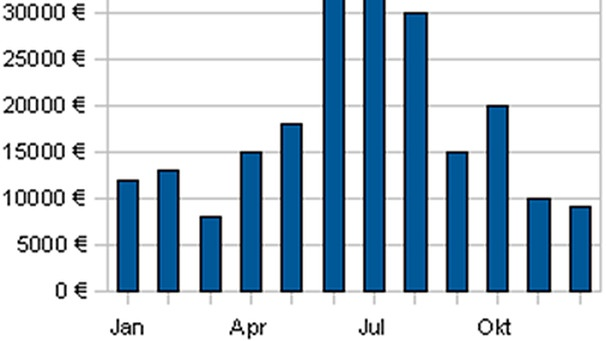
\includegraphics[width=\textwidth]{src/assets/some_graph}
	\caption{Einbinden einer Beispiel-Grafik}
	\label{fig:anylabel}
\end{figure}

Die Grafiken werden automatisch nummeriert, brauchen jedoch ein eindeutig identifizierbares Label, um
solche Grafiken referenzieren zu können.